\begin{titlepage}
\setcounter{page}{0}
\newcommand{\HRule}{\rule{\linewidth}{0.5mm}} % Defines a new command for the horizontal lines, change thickness here

\center % Center everything on the page
 

\includegraphics[scale=0.1]{figs/GlaLogo.pdf}\\[0.5cm]

\vspace{1cm}
\textsc{\LARGE ENG5026: Design Special Topic 5}\\[0.5cm] 
\textsc{\Large Final Report}\\[0.5cm]


\HRule \\[0.4cm]
{ \huge \bfseries WIFI-HIFI \\
\vspace{0.5cm}
\large A wireless, multi-channel audio system.}\\[0.3cm] % Title of your document
\HRule \\[1.5cm]
 
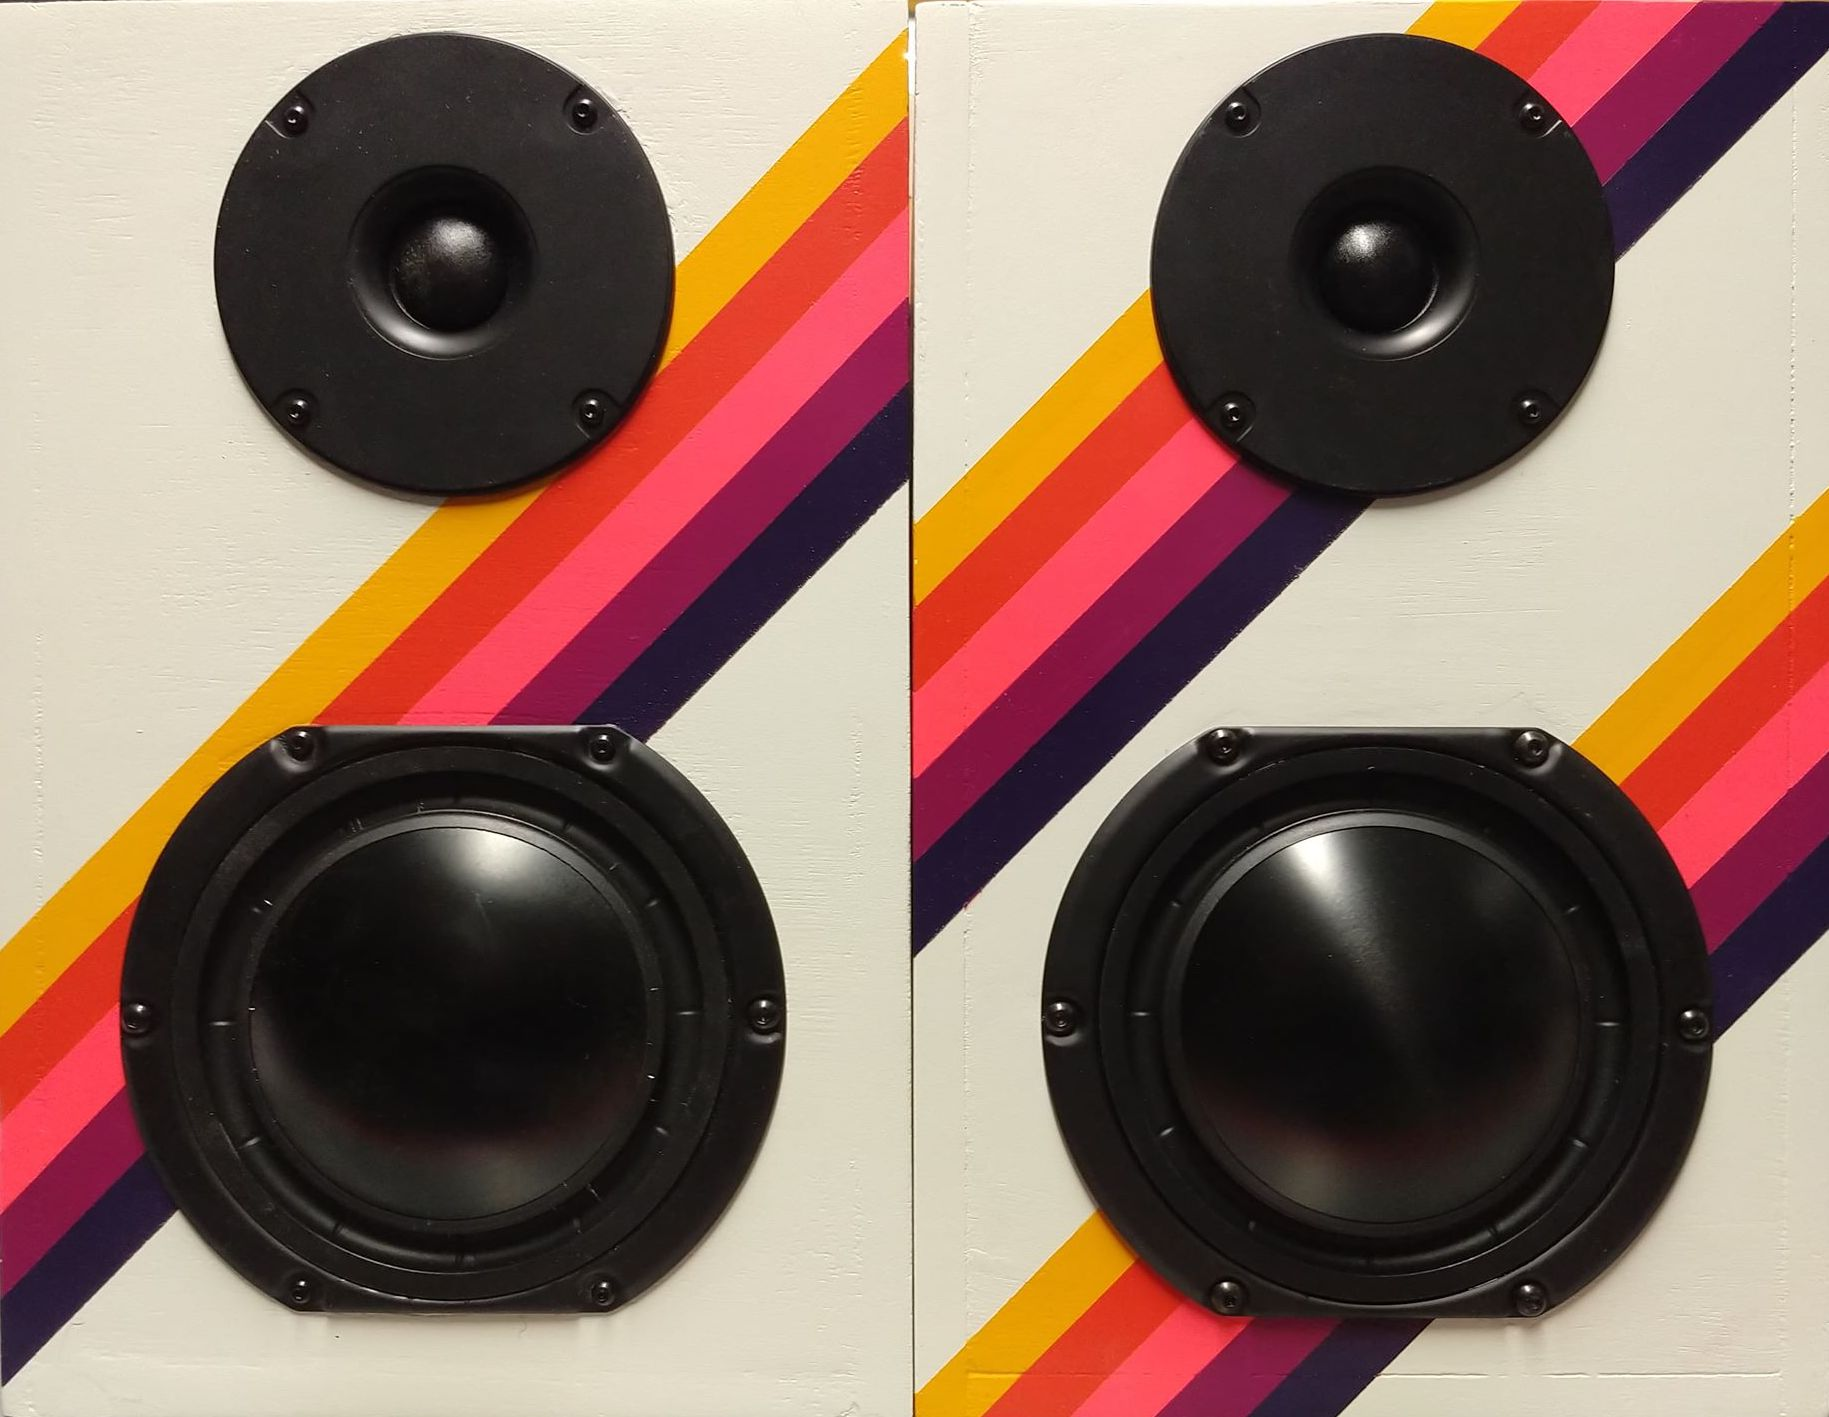
\includegraphics[scale=0.1]{./figs/speakersFront.jpg}\\[0.5cm]

\vspace{1cm}
 
%----------------------------------------------------------------------------------------
%	AUTHOR SECTION
%----------------------------------------------------------------------------------------

\begin{minipage}[t]{0.4\textwidth}
\begin{flushleft} \large
\emph{Authors:}\\
Jamie \textsc{Brown} % Your name

Peter \textsc{Fleming} % Supervisor's Name

Eoin \textsc{McKiernan}
\end{flushleft}
\end{minipage}
~
\begin{minipage}[t]{0.4\textwidth}
\begin{flushright} \large
\emph{Supervisor:} \\
Professor. Scott \textsc{Roy} % Supervisor's Name

\end{flushright}
\end{minipage}\\[2cm]

{\large \today}\\[2cm] % Date, change the \today to a set date if you want to be precise

\vfill % Fill the rest of the page with whitespace

\end{titlepage}